%-*-latex-*-
\sectionthree{Traversal}
\begin{python0}
from solutions import *; clear()
\end{python0}

When you have an array, vector or a linked list,
you can \lq\lq travel through'' (or to traverse) the container 
from the front to the back or the back to the front
for instance when you want to print the contents of the 
container or when you want to search for a value.

In the case of a tree, there are many more ways to traverse
the container.
I'm going to focus on binary trees since it's the easiest case.
Let me illustrate 4 different traversals using this example:

\begin{center}
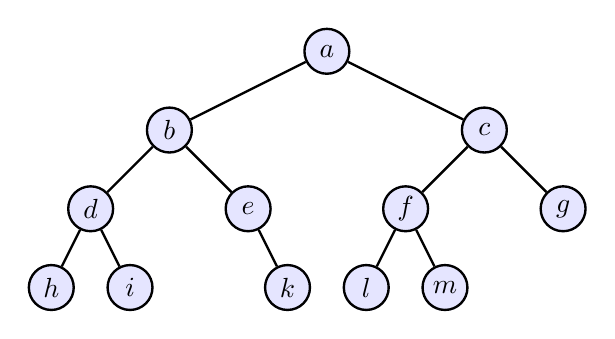
\begin{tikzpicture}

\fill[blue!10] (0.0, 0.0) circle (0.3);
\node [line width=0.03cm,black,minimum size=0.57cm,draw,circle] at (0.0,0.0)(a){};\draw (0.0, 0.0) node[color=black] {$a$};
\fill[blue!10] (-2.0, -1.0) circle (0.3);
\node [line width=0.03cm,black,minimum size=0.57cm,draw,circle] at (-2.0,-1.0)(b){};\draw (-2.0, -1.0) node[color=black] {$b$};
\fill[blue!10] (2.0, -1.0) circle (0.3);
\node [line width=0.03cm,black,minimum size=0.57cm,draw,circle] at (2.0,-1.0)(c){};\draw (2.0, -1.0) node[color=black] {$c$};
\fill[blue!10] (-3.0, -2.0) circle (0.3);
\node [line width=0.03cm,black,minimum size=0.57cm,draw,circle] at (-3.0,-2.0)(d){};\draw (-3.0, -2.0) node[color=black] {$d$};
\fill[blue!10] (-1.0, -2.0) circle (0.3);
\node [line width=0.03cm,black,minimum size=0.57cm,draw,circle] at (-1.0,-2.0)(e){};\draw (-1.0, -2.0) node[color=black] {$e$};
\fill[blue!10] (1.0, -2.0) circle (0.3);
\node [line width=0.03cm,black,minimum size=0.57cm,draw,circle] at (1.0,-2.0)(f){};\draw (1.0, -2.0) node[color=black] {$f$};
\fill[blue!10] (3.0, -2.0) circle (0.3);
\node [line width=0.03cm,black,minimum size=0.57cm,draw,circle] at (3.0,-2.0)(g){};\draw (3.0, -2.0) node[color=black] {$g$};
\fill[blue!10] (-3.5, -3.0) circle (0.3);
\node [line width=0.03cm,black,minimum size=0.57cm,draw,circle] at (-3.5,-3.0)(h){};\draw (-3.5, -3.0) node[color=black] {$h$};
\fill[blue!10] (-2.5, -3.0) circle (0.3);
\node [line width=0.03cm,black,minimum size=0.57cm,draw,circle] at (-2.5,-3.0)(i){};\draw (-2.5, -3.0) node[color=black] {$i$};
\fill[blue!10] (-0.5, -3.0) circle (0.3);
\node [line width=0.03cm,black,minimum size=0.57cm,draw,circle] at (-0.5,-3.0)(k){};\draw (-0.5, -3.0) node[color=black] {$k$};
\fill[blue!10] (0.5, -3.0) circle (0.3);
\node [line width=0.03cm,black,minimum size=0.57cm,draw,circle] at (0.5,-3.0)(l){};\draw (0.5, -3.0) node[color=black] {$l$};
\fill[blue!10] (1.5, -3.0) circle (0.3);
\node [line width=0.03cm,black,minimum size=0.57cm,draw,circle] at (1.5,-3.0)(m){};\draw (1.5, -3.0) node[color=black] {$m$};\draw[line width=0.03cm,black] (a) to  (b);
\draw[line width=0.03cm,black] (a) to  (c);
\draw[line width=0.03cm,black] (b) to  (d);
\draw[line width=0.03cm,black] (b) to  (e);
\draw[line width=0.03cm,black] (c) to  (f);
\draw[line width=0.03cm,black] (c) to  (g);
\draw[line width=0.03cm,black] (d) to  (h);
\draw[line width=0.03cm,black] (d) to  (i);
\draw[line width=0.03cm,black] (e) to  (k);
\draw[line width=0.03cm,black] (f) to  (l);
\draw[line width=0.03cm,black] (f) to  (m);
\end{tikzpicture}

\end{center}



The first three are called \defone{depth first} (DF) traversals because 
they tend to dive deep down into the tree quickly.
The last one is called \defone{breadth first} (BF) traversal
before you go down one level at a time.


\begin{itemize}

\li DF: Pre-order traversal:
Here's a memory aid: \lq\lq root, left, right''.
Here is the printing of the node  of the above tree using
pre-order traversal:
\[
a, b, d, h, i, e, k, c, f, l, m, g
\]

\li DF: In-order traversal:
In this case you do \lq\lq left, root, right''.
Here's the printing of the above tree using this method of traversal:
\[
h, d, i, b, e, k, a, l, f, m, c, g
\]

\li DF: Post-order traversal:
And for this one, use \lq\lq left, right, root:
\[
h, i, d, k, e, b, l, m, f, g, c, a
\]

\li BF: 
Breadth-first goes through the tree one level at a time.
Here's the printing the tree using breadth first traversal:
\[
a, b, c, d, e, f, g, h, i, k, l, m
\]
In this case, we are scanning left-to-right for each level.
The important is that all the nodes are processed at a level
before going down to the next level.
\end{itemize}

(There are actually many other traversals. 
You can come across them if you take the AI class, 
different traversals will impact the performance of the  
algorithms that search for an intelligent solutions.)

Here's the pseudocode for the first DF traversal:
\begin{console}
PREORDER-PRINT
INPUT: p = pointer to root of a tree

if p is NULL: 
    return
else:
    print p->key
    PREORDER-PRINT(p->left)
    PREORDER-PRINT(p->right)
\end{console}
This version uses recursion.
Here's a version that uses a stack instead:
\begin{console}
PREORDER-PRINT
INPUT: p = pointer to root of a tree

if p is NULL:
    return

let s = empty stack of pointer to node
push p onto s

while s is not empty:
    x = s.pop()
    print x->key
    if x->right is not NULL:
        push x->right onto s
    if x->left is not NULL:
        push x->left onto s
\end{console}
It's clear what the pseudocode for inorder and postorder 
should look like.
In the above, NULL pointers are not inserted into the stack.
If we do allow NULL pointers in the stack, then the pseudocode would look
like this:
\begin{console}
PREORDER-PRINT
INPUT: p = pointer to root of a tree

let s = empty stack of pointer to node
push p onto s

while s is not empty:
    x = s.pop()
    if x is not NULL:
        print x->key
        push x->right onto s
        push x->left onto s
\end{console}
which is simpler.



For the BF traversal, you use a queue instead of a stack,
and do this:
\begin{Verbatim}[frame=single,commandchars=\\\{\}]
BREADTH-FIRST-PRINT
INPUT: p = pointer to root of a tree

if p == NULL:
    return 

let q = empty queue of pointers to node
q.enqueue(p)

while q is not empty:
    x = q.dequeue()
    print x->key
    if x->left is not NULL:
        put x->left into q
    if x->right is not NULL:
        put x->right into q  
\end{Verbatim}
This version does not put NULL pointers into the stack.
If you allow NULL pointers in the stack, then:
\begin{Verbatim}[frame=single,commandchars=\\\{\}]
BREADTH-FIRST-PRINT
INPUT: p = pointer to root of a tree

let q = empty queue of pointers to node
q.enqueue(p)

while q is not empty:
    x = q.dequeue()
    if x is not NULL:
        print x->key
        put x->left into q
        put x->right into q  
\end{Verbatim}
which is simpler.
